\documentclass[10pt,a4paper]{article}
\usepackage[utf8]{inputenc}
\usepackage[french]{babel}
\usepackage[T1]{fontenc}
\usepackage{amsmath}
\usepackage{amsfonts}
\usepackage{amssymb}
\usepackage{makeidx}
\usepackage{xcolor} 
\usepackage{graphicx}
\usepackage{lmodern}
\usepackage[many]{tcolorbox}
\usetikzlibrary{shadows}
\usepackage{kpfonts}
\usepackage{geometry}
\usepackage{xcolor} 
\usepackage{fancybox}
\usepackage{graphicx}
\usepackage{lmodern}
\author{KOUTEMA Ditoma}

\begin{document}
\newtcolorbox{shadedbox}{
  drop shadow southeast,
  breakable,
  enhanced jigsaw,
  colback=white,
}

\begin{shadedbox}
\begin{center}
\huge \textcolor{blue}{TP03 Python Django – Shell et site d'administration}
\end{center}
\end{shadedbox}
%fin box%
\large{\begin{center}
fait par : 
\end{center}}
\begin{center}
\huge{KOUTEMA Ditoma}
\end{center}
\newpage
\tableofcontents
\newpage

\section{Mise en route}
Pour travailler dans les bonnes conditions, je suis rentré dans mon projet et j'ai fait un clic droit et en suite j'ai ouvert le terminal a partir de la. Puis j'ai lancer le serveur de développement comme suit : \textcolor{blue}{py manage.py runserver}

\section{L'interface de programmation (API)}
\begin{enumerate}
\item 
\begin{itemize}
\item[]
\item[•] \textbf{API :}  Application Programming Interface.
\item[•] L'api permet a deux applications distinctes des communiquer et d'échanger des données.
\item[•] Un shell est un interpréteur de commandes destiné aux systèmes d'exploitation de type linux qui permet d'accéder aux fonctionnalités internes du système d'exploitation.
\end{itemize}


\item 
\begin{itemize}
\item[]
\item[•] Quand on lance la commande : \textcolor{blue}{py manage.py shell}, il ouvre le shell de python avec sa version installé. \\
\begin{verbatim}
Python 3.10.12 (main, Jun 11 2023, 05:26:28) [GCC 11.4.0] on linux
Type "help", "copyright", "credits" or "license" for more information.
(InteractiveConsole)
>>> 
\end{verbatim}

\item[•] Quand je lance la commande alias seule : \textcolor{blue}{py}\\
\begin{verbatim}
Python 3.10.12 (main, Jun 11 2023, 05:26:28) [GCC 11.4.0] on linux
Type "help", "copyright", "credits" or "license" for more information.
>>> 
\end{verbatim}

\item[•] Donc la différence entre \textcolor{blue}{py manage.py shell} et \textcolor{blue}{py} : Avec la première commande il y a l'information \textcolor{blue}{(InteractiveConsole)} qui s'ajoute dans le shell python. Le fichier utilisé dans le prémier cas est \textcolor{blue}{manage.py}
\end{itemize}



\item 
\begin{itemize}
\item[]
\item[a)] Pour voir ce que contient l'attribut je me suis servie de l'extension de visual studio code qui s’appelle \textcolor{blue}{sqlite viewer}. Ici l'attribut ne contient rien.\\\\
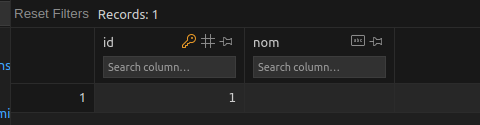
\includegraphics[scale=0.6]{1.png}
\item[•] Oui c'est normal.
\item[•] Il n'y a pas d'erreur car il est unique ce qui veut dire qu'il peut donc être \textcolor{blue}{null}\\

\item[b)] Création du niveau2 : \\
\begin{verbatim}
>>> from notes.models import *

>>> niveau2 = Niveau()
>>> niveau2.save()

\end{verbatim}
\item[•] Après la sauvegarde de l'objet niveau2 il y a une erreur qui s'est produite.
\item[•] Cette erreur est du a la violation de la contrainte unique.\\

\item[c)] Suppression du niveau sauvegardé dans la base de donnée : \\
\item[•]On doit selectionner DImdjflkl'objet d'abord et en suite le supprimer.\\
\begin{verbatim}
>>> niveau = Niveau.objects.get(pk=1)
>>> niveau.delete()
(1, {'notes.Niveau': 1})
>>> 
\end{verbatim}
\item[•] Pour preuve je vais retourner sur visual studio code et me servir de sqlite. viewer.\\\\
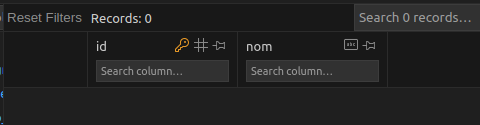
\includegraphics[scale=0.6]{2.png}


\item[d)] Création des niveaux : \\\\
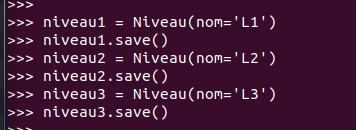
\includegraphics[scale=0.8]{n1.png}
\item[•] Valeurs des clés primaire: 2, 3, 4\\\\
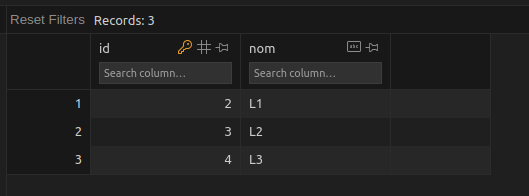
\includegraphics[scale=0.5]{3.png}\\

\item[e)] Création de 4 Élevés : \\
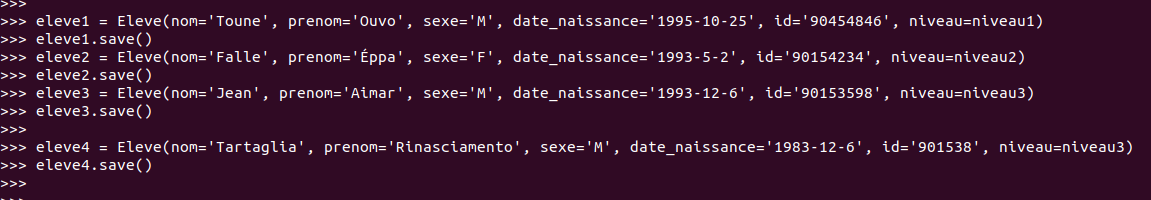
\includegraphics[scale=0.3]{n2.png}
\end{itemize}

\item[f)] Créations de trois enseignants.\\\\
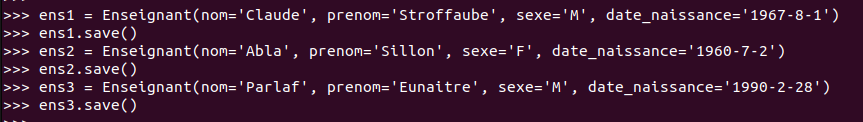
\includegraphics[scale=0.5]{n3.png}


\item[g)] Créations de 5 matières.\\\\
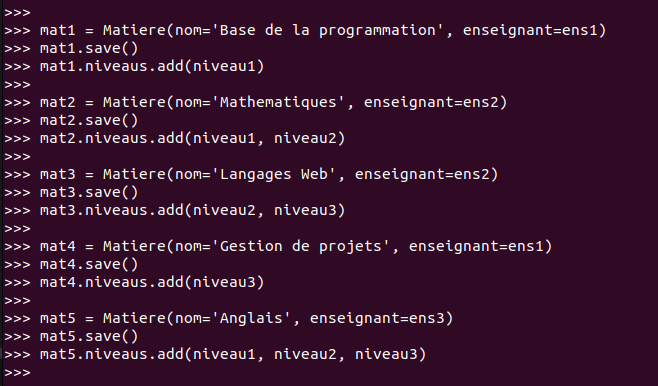
\includegraphics[scale=0.5]{n4.png}\\



\item 
\begin{itemize}
\item[]

\item[•]Affichons l'objet Élevé correspondant a 'Jean'.\\\\
\begin{verbatim}
>>> print(Eleve.objects.get(nom='Jean'))
Eleve object (90153598)
>>> 
\end{verbatim}
\item[•] Ce qui s'affiche c'est la classe Élevé, sont type et sa clé primaire.
Voilà donc comment voire sa .

\item[•] Oui se serait mieux. Donc pour le faire, je crée la méthode spécial \_\_str\_\_ dans mon modèle qui retourne le nom et le prénom comme suit: \\

\begin{verbatim}
def __str__(self):
        return self.nom + " " + self.prenom
\end{verbatim}

\item[•] Code
\begin{verbatim}
from django.db import models

# Create your models
 here.
class Personne(models.Model):
    nom = models.CharField(max_length=50)
    prenom = models.CharField(max_length=50)
    sexe = models.CharField(max_length=100, 
    choices=(('M', 'Masculin'),('F', 'Feminin'))) 
    date_naissance = models.DateField()

    class Meta:
        abstract = True


class Niveau(models.Model):
    nom = models.CharField(max_length=2, unique=True)

    def __str__(self):
        return self.nom
    


class Enseignant(Personne):
    def __str__(self):
        return self.nom + " " + self.prenom +" "+ self.sexe + 
        " " + self.date_naissance


class Matiere(models.Model):
    nom = models.CharField(max_length=50, unique=True)
    enseignant = models.ForeignKey(Enseignant, 
    on_delete=models.CASCADE)
    niveaus = models.ManyToManyField(Niveau)

    def __str__(self):
        return self.nom + " " + self.enseignant

    


class Eleve(Personne):
    id=models.BigAutoField(primary_key=True)
    niveau = models.ForeignKey(Niveau, on_delete=models.CASCADE)
    matieres = models.ManyToManyField(Matiere)

    def __str__(self):
        return self.nom + " " + self.prenom


class Note(models.Model):
    eleve = models.ForeignKey(Eleve, on_delete=models.CASCADE)
    valeur = models.FloatField(max_length=30, null=True)

    def __str__(self):
        return self.eleve + " " + self.valeur

\end{verbatim}
\end{itemize}


\item
\begin{itemize}
\item[•]
\item Brrrrrrrrrrrrrrrrrrrrrrrrr!!!!!!!!!!!!!!!
\end{itemize}

\end{enumerate}

\section{Le site d'administration}

\begin{enumerate}

\item 
\begin{itemize}
\item[] La commande pour créer un super utilisateur :  \textcolor{blue}{py manage.py createsuperuser}


\end{itemize}

\item
\begin{itemize}
\item[•] D'abord je demarre le serveur sur le port 8000 : \textcolor{blue}{py manage.py runserver localhost:8000}.
\item[•] En suite je fais clique droit sur le lien et j'ouvre un onglet dans le navigateur.
\item[•] Comme j'ai déjà créer un super utilisateur alors on me demande de m'authentifier.

\item[•] Pour mettre l'application en français alors allez dans le fichier \textcolor{blue}{setting.py} du projet et modifier la ligne suivante : \textcolor{blue}{LANGUAGE\_CODE = 'fr-FR'}
\end{itemize}

Fixons les attributs qui seront visible par l'utilisateur
\item
\begin{itemize}
\item[•] Le fichier \textcolor{blue}{notes/admin.py} nous permet d'enregistrer nos tables.
\item[•] La ligne qu'il faut ajouter est une importation des modèles à utiliser.\\\\
\textcolor{blue}{from notes.models import  Eleve, Enseignant, Matiere, Niveau}

\large{Report du code :}
\begin{verbatim}

from django.contrib import admin
from notes.models import  Eleve, Enseignant, Matiere, Niveau
# Register your models here.

admin.site.register(Niveau)
admin.site.register(Eleve)
admin.site.register(Enseignant)
admin.site.register(Matiere)
\end{verbatim}

Ce qu'on obtient comme résultat : \\\\
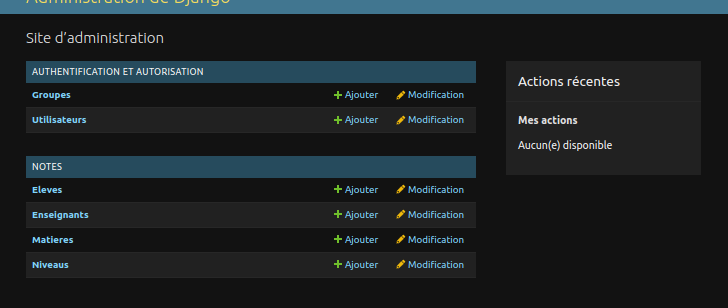
\includegraphics[scale=0.5]{r1.png}
\end{itemize}


\item
\begin{itemize}
\item Oui il y a une erreur au niveau du modèle Élève, car il n'y pas d'accent.\\
\item Pour remédier a ce problème, on ajoute ce morceau de code suivant : 
\begin{verbatim}
class Meta:
        verbose_name_plural = 'Élève'
\end{verbatim}
\end{itemize}



\end{enumerate}






















\end{document}